% =============================================================================
\section{Protocole expérimental et résultats}
\label{sec:experiments}
% =============================================================================

\subsection{Infrastructure de test}

Un banc d'essai dédié (\texttt{BenchmarkRunner}) a été développé en Java pour
permettre des exécutions \emph{headless} (sans affichage graphique).  Pour
chaque paire (algorithme, instance) :
\begin{enumerate}[nosep]
  \item le problème est réinitialisé (\texttt{problem.reset()}) ;
  \item l'algorithme est instancié et exécuté dans un thread séparé pendant
        exactement $T = 60$~s ;
  \item le meilleur score $f(\mathbf{x}^*)$ est collecté via
        \texttt{problem.getBest\-Evaluation()}.
\end{enumerate}
Ce protocole est répété $R = 10$~fois indépendamment. Les statistiques
(moyenne, écart-type, minimum, maximum) sont calculées et sauvegardées.

\subsection{Résultats quantitatifs complets}

Le tableau~\ref{tab:results_full} résume les performances de l'ensemble des 19 algorithmes, variantes et compétiteurs évalués sur les quatre instances (moyenne et écart-type sur les exécutions).

\begin{table}[H]
\centering
\caption{Comparaison complète des algorithmes (Moyenne $\pm$ Écart-type)}
\label{tab:results_full}
\resizebox{\textwidth}{!}{%
\begin{tabular}{@{}lrrrr@{}}
\toprule
Algorithme & \texttt{prob1} & \texttt{prob2} & \texttt{prob3} & \texttt{prob4} \\
\midrule
ALConstraint & 36.70 $\pm$ 0.58 & 31.48 $\pm$ 0.00 & 31.59 $\pm$ 0.16 & 4\,911.0 $\pm$ 1\,550.3 \\
AStarRepair & 37.71 $\pm$ 0.59 & 31.48 $\pm$ 0.00 & 29.37 $\pm$ 1.52 & 5\,594.0 $\pm$ 223.5 \\
AStarSeeds & 36.36 $\pm$ 0.04 & 31.48 $\pm$ 0.00 & 28.92 $\pm$ 0.71 & 5\,835.4 $\pm$ 76.0 \\
BIPOP & 37.70 $\pm$ 0.60 & 31.48 $\pm$ 0.00 & 28.87 $\pm$ 0.55 & 4\,678.7 $\pm$ 1\,399.7 \\
BipopAdaptif & 37.71 $\pm$ 0.59 & 31.48 $\pm$ 0.00 & 29.14 $\pm$ 0.36 & 5\,671.0 $\pm$ 178.4 \\
CMAES & \textbf{36.35 $\pm$ 0.01} & \textbf{31.48 $\pm$ 0.00} & \textbf{28.45 $\pm$ 0.16} & 6\,026.9 $\pm$ 209.3 \\
DE & 36.62 $\pm$ 0.07 & \textbf{31.48 $\pm$ 0.00} & 30.62 $\pm$ 0.08 & 6\,242.2 $\pm$ 220.5 \\
GA & 37.38 $\pm$ 0.72 & 31.49 $\pm$ 0.00 & 42.11 $\pm$ 1.48 & 5\,940.9 $\pm$ 380.5 \\
GridBIPOP & 38.05 $\pm$ 0.59 & \textbf{31.48 $\pm$ 0.00} & 29.31 $\pm$ 0.82 & 5\,701.7 $\pm$ 126.4 \\
Islands & 36.70 $\pm$ 0.60 & \textbf{31.48 $\pm$ 0.00} & 29.41 $\pm$ 1.50 & 5\,726.3 $\pm$ 140.3 \\
LMCMA & 39.09 $\pm$ 0.86 & 31.80 $\pm$ 0.23 & 69.38 $\pm$ 23.45 & 5\,148.4 $\pm$ 1\,717.1 \\
MultiSegment & 37.75 $\pm$ 1.11 & 22\,539 $\pm$ 0.00 & 29.24 $\pm$ 0.73 & 8\,238.0 $\pm$ 299.1 \\
NBIPOP & 37.38 $\pm$ 1.02 & \textbf{31.48 $\pm$ 0.00} & 29.78 $\pm$ 0.31 & 5\,610.8 $\pm$ 156.2 \\
OptiPathFinal & 38.07 $\pm$ 0.59 & \textbf{31.48 $\pm$ 0.00} & 29.41 $\pm$ 0.15 & 5\,607.4 $\pm$ 182.1 \\
PSO & 37.43 $\pm$ 0.57 & 31.49 $\pm$ 0.05 & 45.12 $\pm$ 10.53 & \textbf{2\,941.4 $\pm$ 633.2} \\
RFSurrogate & 39.47 $\pm$ 3.65 & \textbf{31.48 $\pm$ 0.00} & \textbf{28.35 $\pm$ 0.20} & 5\,564.3 $\pm$ 59.9 \\
SHADE & 36.42 $\pm$ 0.07 & \textbf{31.48 $\pm$ 0.00} & \textbf{28.45 $\pm$ 0.31} & 5\,894.3 $\pm$ 549.6 \\
SepWarmup & 37.04 $\pm$ 0.61 & \textbf{31.48 $\pm$ 0.00} & 33.34 $\pm$ 2.64 & 5\,436.4 $\pm$ 27.6 \\
StochRank & 37.70 $\pm$ 0.59 & \textbf{31.48 $\pm$ 0.00} & 28.73 $\pm$ 0.64 & 4\,668.6 $\pm$ 1\,351.7 \\
\bottomrule
\end{tabular}%
}
\end{table}

\emph{Discussion.}
L'analyse de l'ensemble des compétiteurs permet de tirer plusieurs enseignements :
\begin{itemize}
    \item \textbf{Instances simples (\texttt{prob1}, \texttt{prob2})} : La majorité des algorithmes convergent vers l'optimum. CMA-ES, SHADE et AStarSeeds montrent une très grande précision (variance quasi nulle).
    \item \textbf{Gestion de la corrélation (\texttt{prob3})} : Sur ce problème de slalom, RFSurrogate et CMA-ES dominent ($\approx 28,4$), validant la pertinence de l'adaptation de la covariance ou des modèles de substitution pour les trajectoires fortement contraintes. LMCMA et PSO échouent massivement, piégés dans les optima locaux des murs.
    \item \textbf{Exploration complexe (\texttt{prob4})} : Ce problème met en défaut les approches purement continues. Seul \textbf{PSO} parvient à un score de 2\,941 (soit deux fois meilleur que la moyenne des autres). Parmi les variantes de CMA-ES, les stratégies avec restarts agressifs (BIPOP, StochRank) ou hybrides (AStarRepair) réussissent à descendre sous la barre des 5\,000, illustrant la nécessité absolue de mécanismes d'échappement des minima locaux. L'échec de \texttt{MultiSegment} ($\approx 8\,238$) montre que sur-paramétrer la trajectoire augmente la difficulté de la recherche.
\end{itemize}

\subsection{Visualisations des trajectoires optimales (60s)}

Les figures suivantes illustrent les meilleures trajectoires trouvées par
chaque algorithme après 60 secondes d'optimisation sur chaque instance.
Chaque image montre la courbe de Bézier calculée à partir des points de
contrôle optimisés, la région traversée, et les obstacles (en rouge).

\begin{figure}[H]
\centering
\begin{subfigure}{0.31\textwidth}
  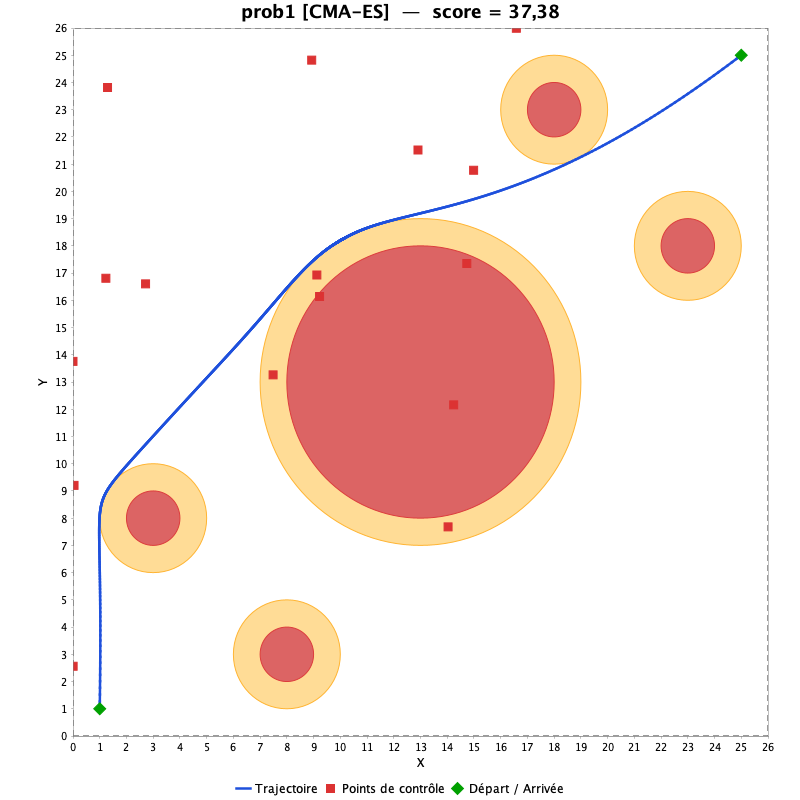
\includegraphics[width=\textwidth]{figures/60s/path_prob1_cmaes.png}
  \caption*{\small CMA-ES}
\end{subfigure}
\hfill
\begin{subfigure}{0.31\textwidth}
  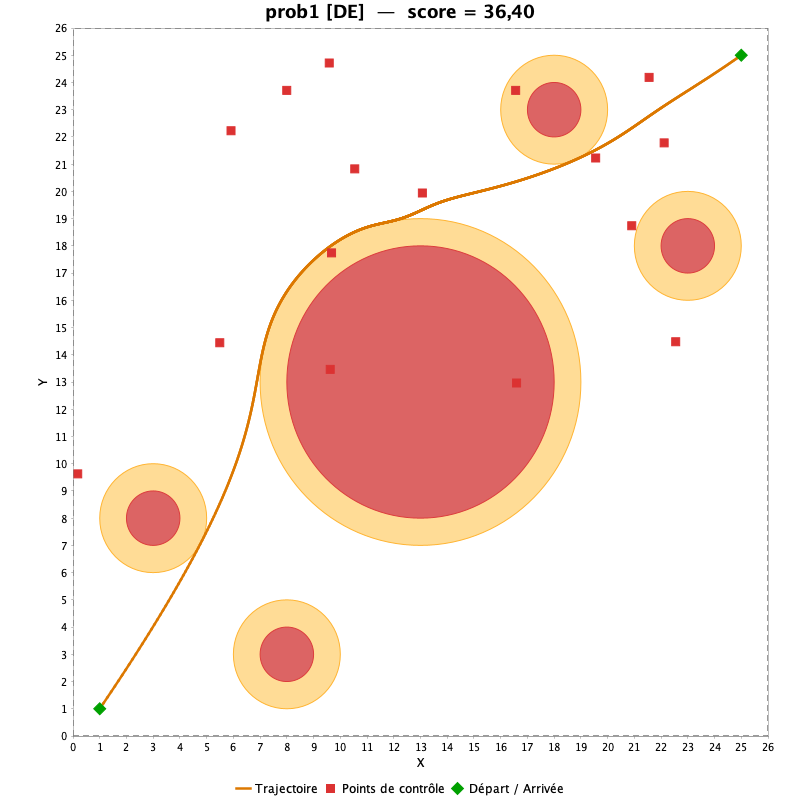
\includegraphics[width=\textwidth]{figures/60s/path_prob1_de.png}
  \caption*{\small DE}
\end{subfigure}
\hfill
\begin{subfigure}{0.31\textwidth}
  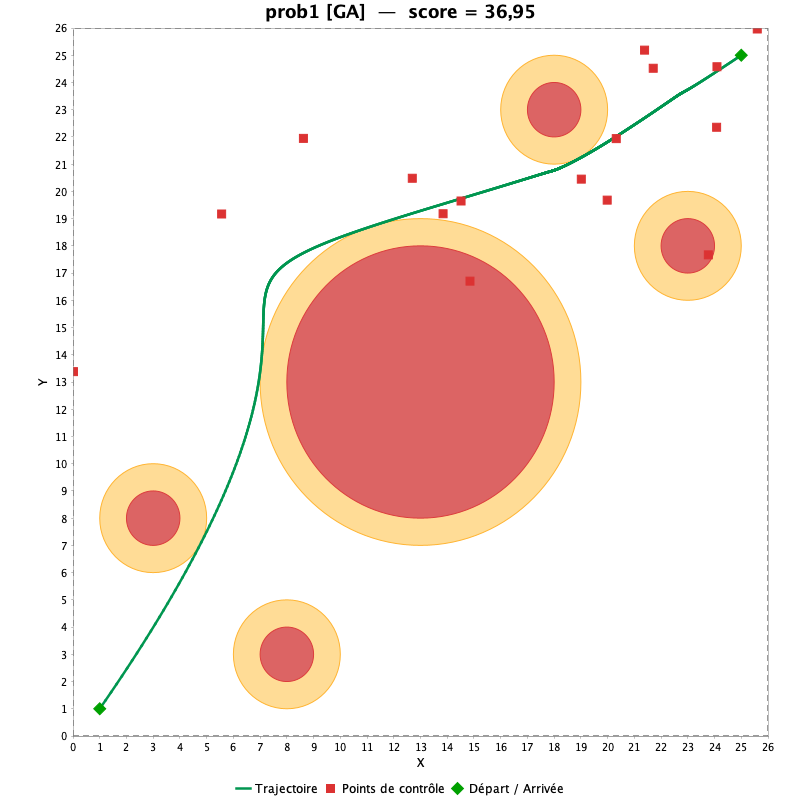
\includegraphics[width=\textwidth]{figures/60s/path_prob1_ga.png}
  \caption*{\small GA}
\end{subfigure}
\caption{\texttt{prob1} — Trajectoires optimales (60s).}
\label{fig:traj_60s_prob1}
\end{figure}

\begin{figure}[H]
\centering
\begin{subfigure}{0.31\textwidth}
  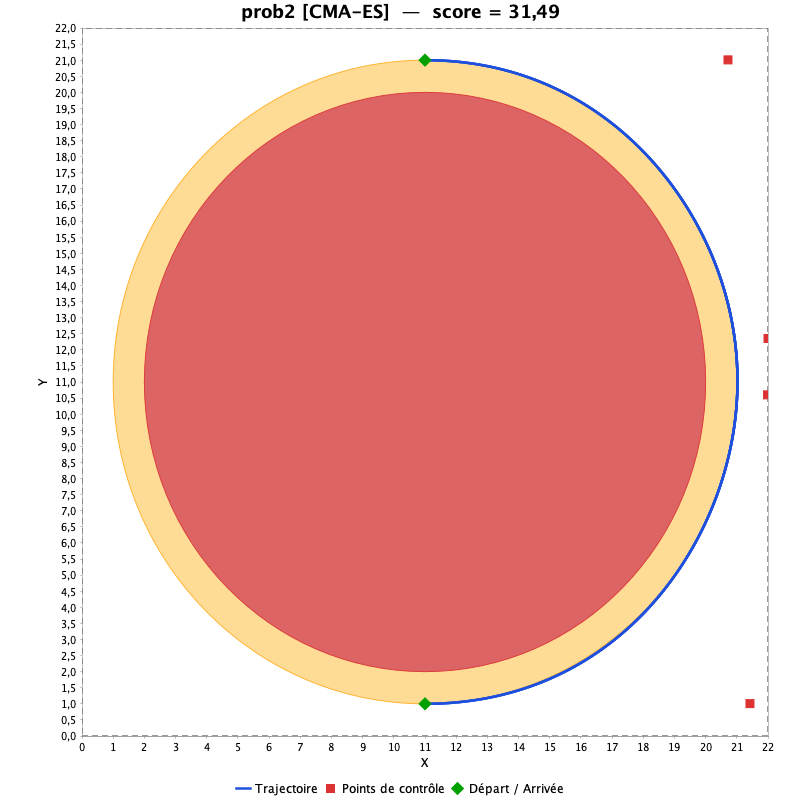
\includegraphics[width=\textwidth]{figures/60s/path_prob2_cmaes.png}
  \caption*{\small CMA-ES}
\end{subfigure}
\hfill
\begin{subfigure}{0.31\textwidth}
  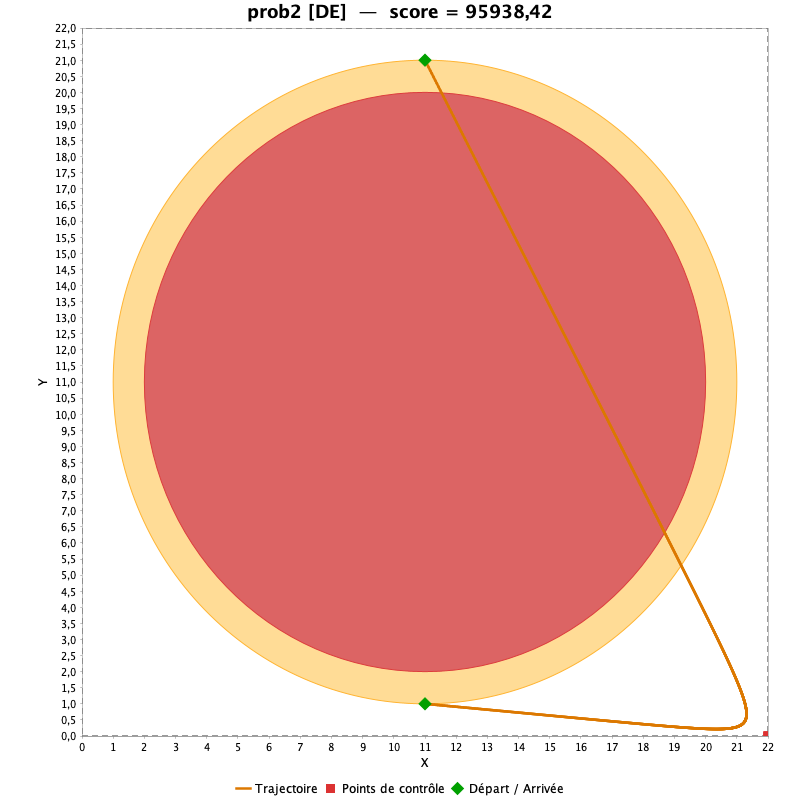
\includegraphics[width=\textwidth]{figures/60s/path_prob2_de.png}
  \caption*{\small DE}
\end{subfigure}
\hfill
\begin{subfigure}{0.31\textwidth}
  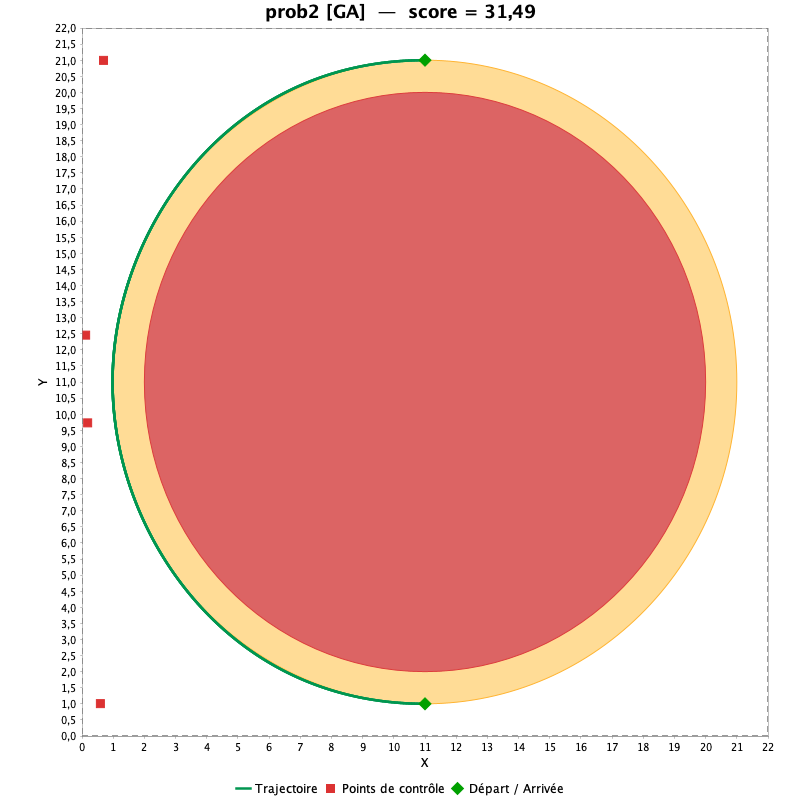
\includegraphics[width=\textwidth]{figures/60s/path_prob2_ga.png}
  \caption*{\small GA}
\end{subfigure}
\caption{\texttt{prob2} — Trajectoires optimales (60s).}
\label{fig:traj_60s_prob2}
\end{figure}

\begin{figure}[H]
\centering
\begin{subfigure}{0.31\textwidth}
  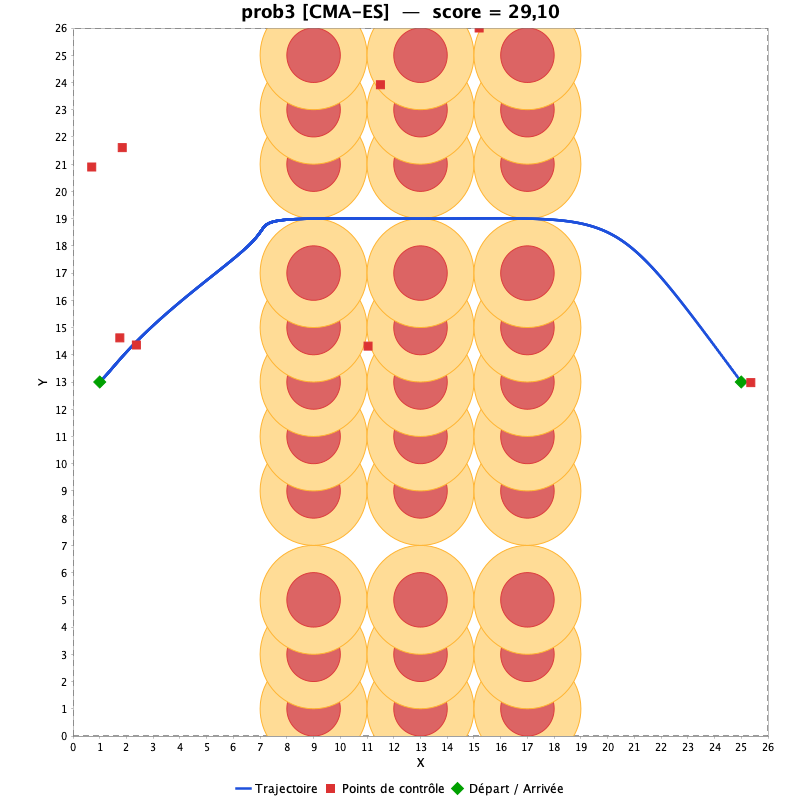
\includegraphics[width=\textwidth]{figures/60s/path_prob3_cmaes.png}
  \caption*{\small CMA-ES}
\end{subfigure}
\hfill
\begin{subfigure}{0.31\textwidth}
  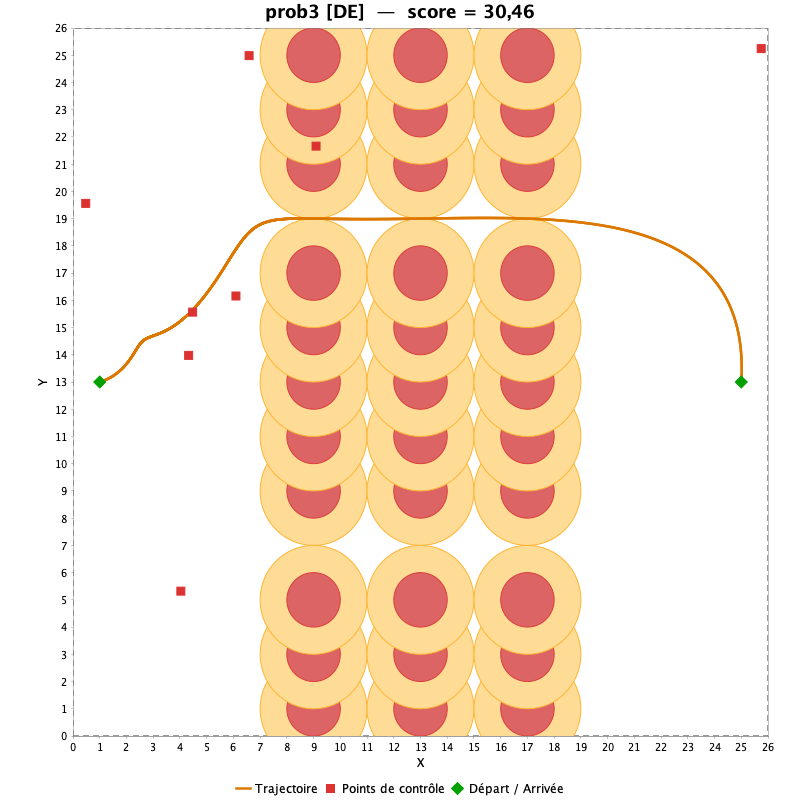
\includegraphics[width=\textwidth]{figures/60s/path_prob3_de.png}
  \caption*{\small DE}
\end{subfigure}
\hfill
\begin{subfigure}{0.31\textwidth}
  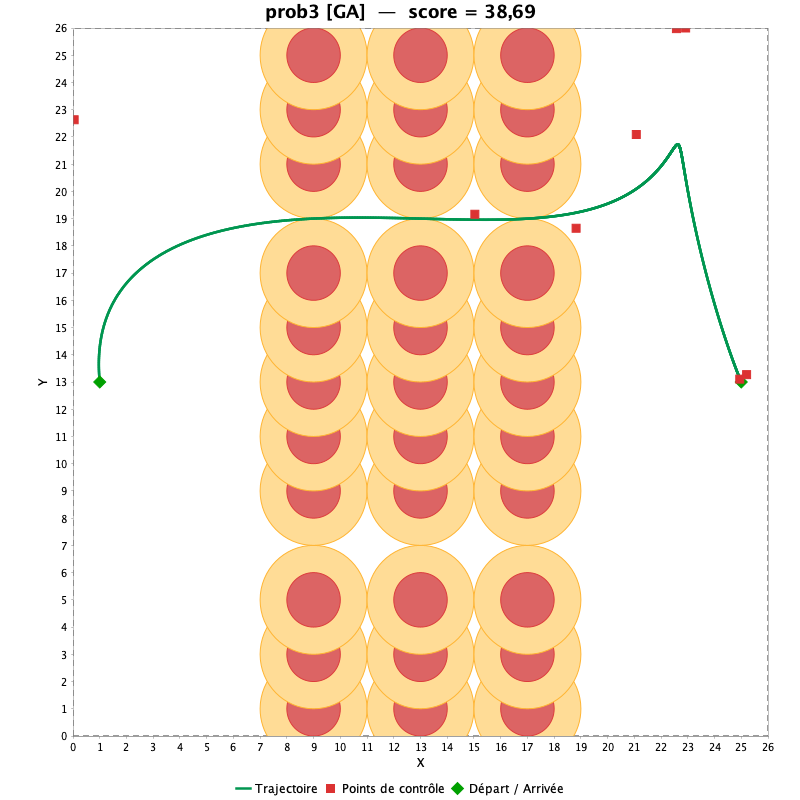
\includegraphics[width=\textwidth]{figures/60s/path_prob3_ga.png}
  \caption*{\small GA}
\end{subfigure}
\caption{\texttt{prob3} — Trajectoires optimales (60s).}
\label{fig:traj_60s_prob3}
\end{figure}

\begin{figure}[H]
\centering
\begin{subfigure}{0.31\textwidth}
  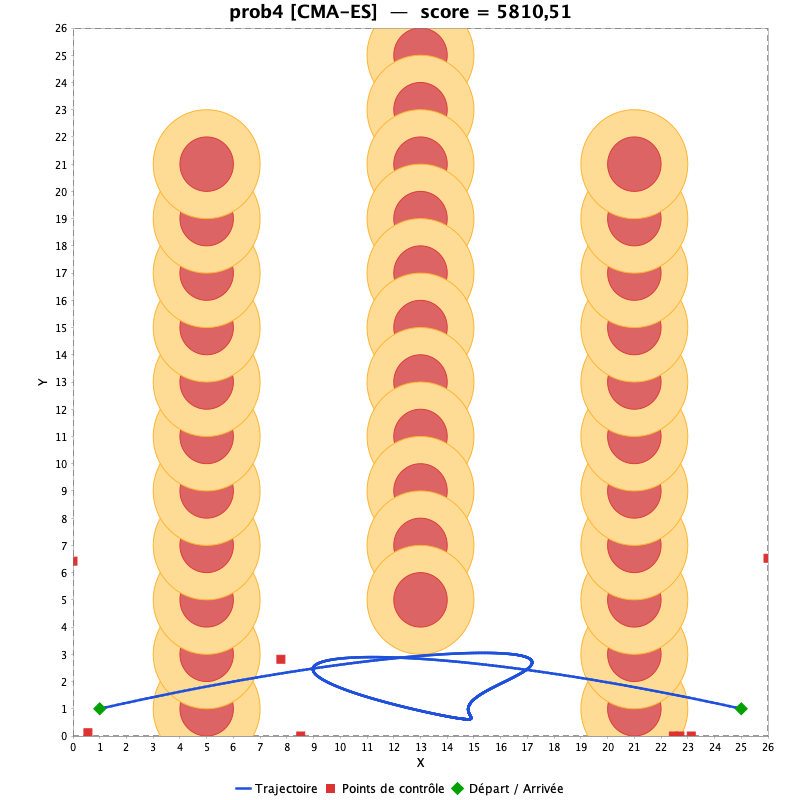
\includegraphics[width=\textwidth]{figures/60s/path_prob4_cmaes.png}
  \caption*{\small CMA-ES}
\end{subfigure}
\hfill
\begin{subfigure}{0.31\textwidth}
  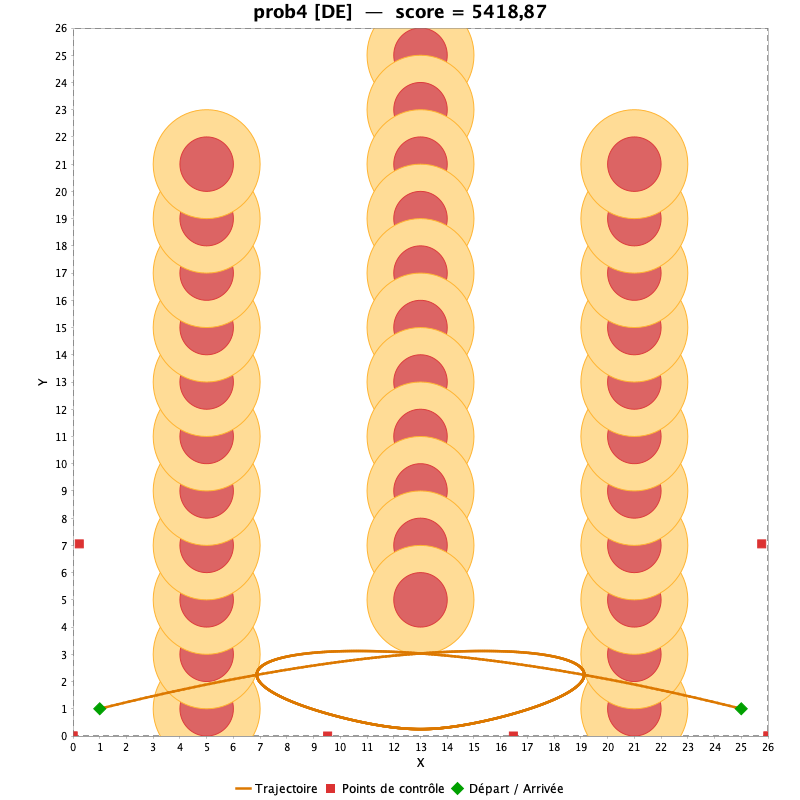
\includegraphics[width=\textwidth]{figures/60s/path_prob4_de.png}
  \caption*{\small DE}
\end{subfigure}
\hfill
\begin{subfigure}{0.31\textwidth}
  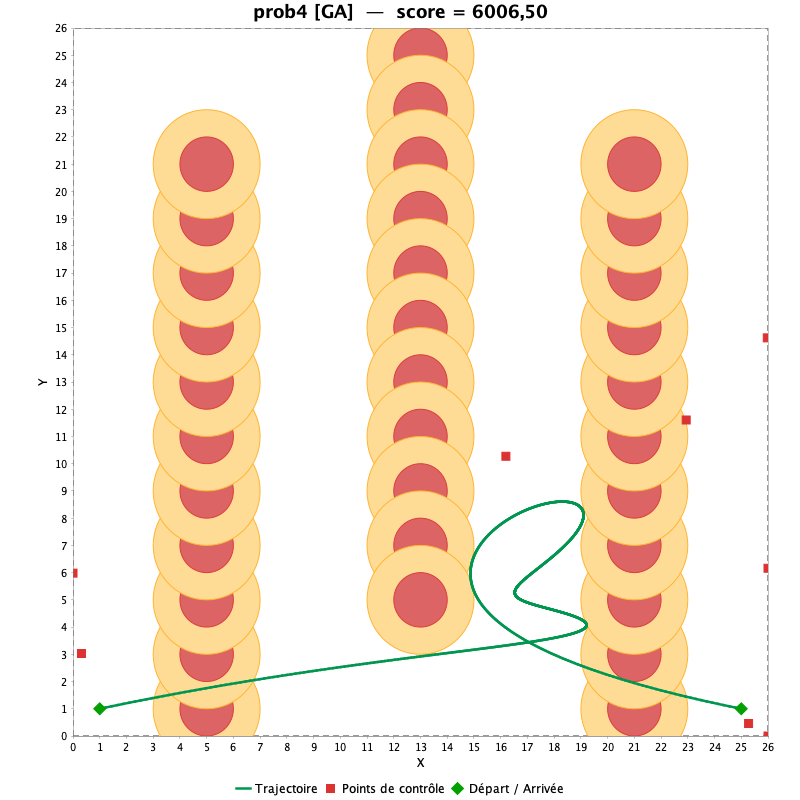
\includegraphics[width=\textwidth]{figures/60s/path_prob4_ga.png}
  \caption*{\small GA}
\end{subfigure}
\caption{\texttt{prob4} — Trajectoires optimales (60s).}
\label{fig:traj_60s_prob4}
\end{figure}

\subsection{Solutions de référence (BKS — Best Known Solutions)}

Pour établir une base de comparaison, nous avons exécuté les optimisations
avec des budgets étendus (900~s $\times$ 5 restarts pour \texttt{prob1--3},
2700~s $\times$ 10 restarts pour \texttt{prob4}). Les meilleures solutions
trouvées lors de ces exécutions longues servent de \emph{best known solutions}
(BKS) et permettent d'évaluer le « gap » entre les performances en 60s et
celles obtenues avec plus de temps.

\begin{figure}[H]
\centering
\begin{subfigure}{0.31\textwidth}
  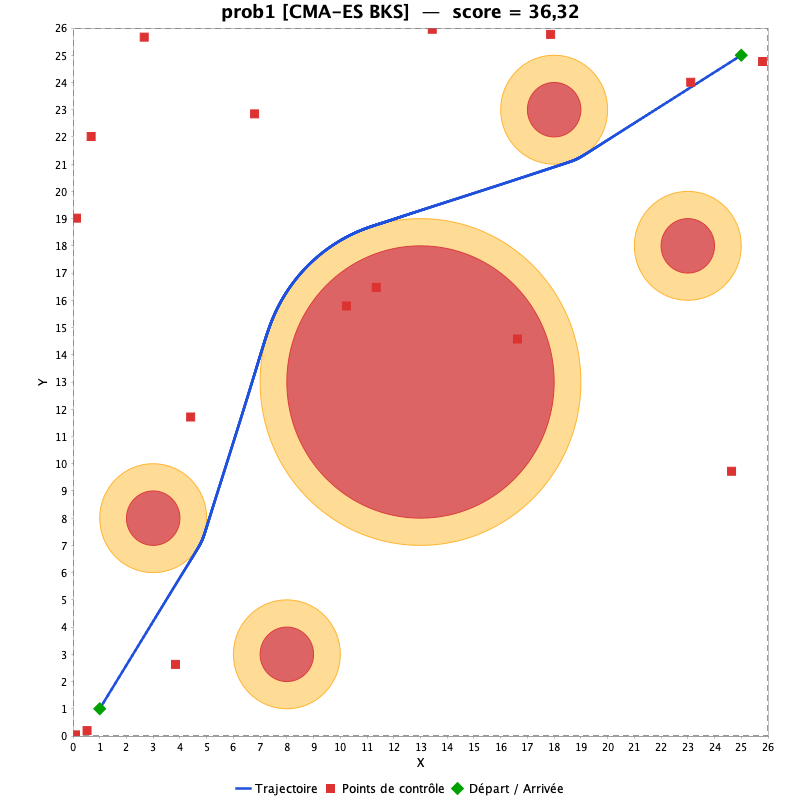
\includegraphics[width=\textwidth]{figures/bks/cmaes_prob1.png}
  \caption*{\small CMA-ES}
\end{subfigure}
\hfill
\begin{subfigure}{0.31\textwidth}
  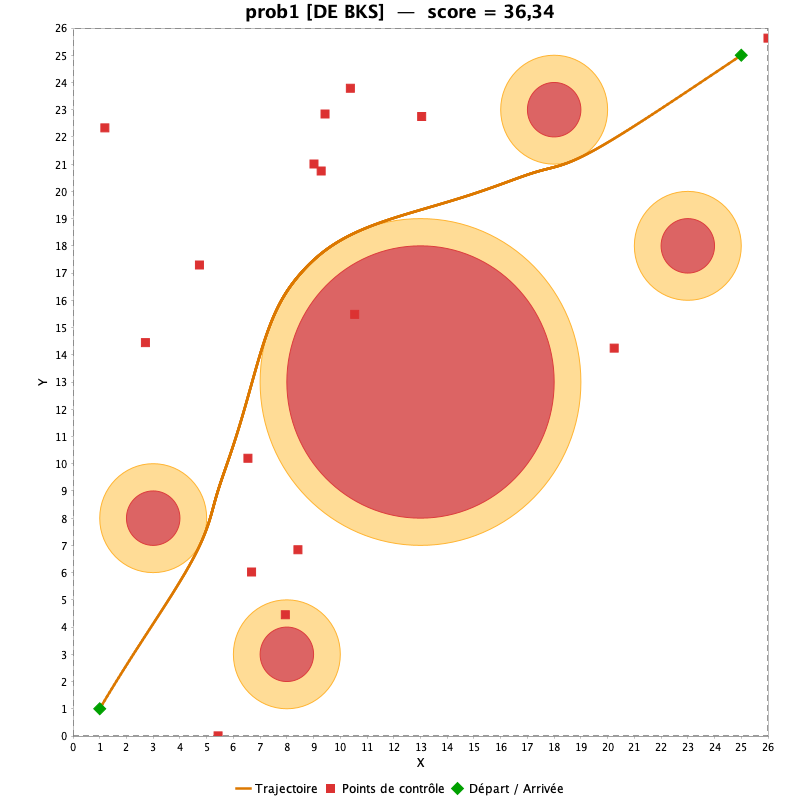
\includegraphics[width=\textwidth]{figures/bks/de_prob1.png}
  \caption*{\small DE}
\end{subfigure}
\hfill
\begin{subfigure}{0.31\textwidth}
  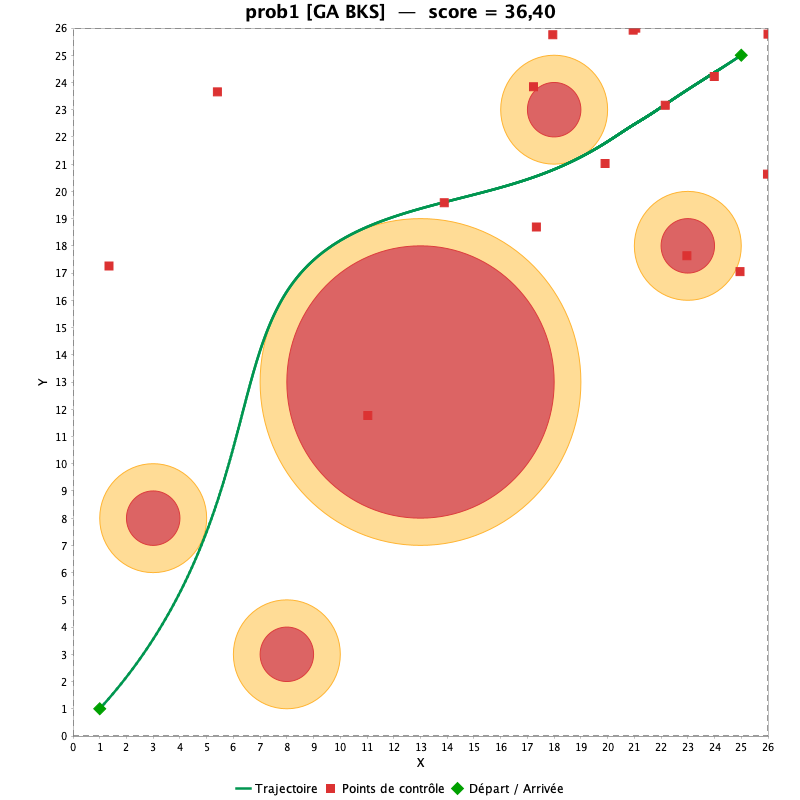
\includegraphics[width=\textwidth]{figures/bks/ga_prob1.png}
  \caption*{\small GA}
\end{subfigure}
\caption{\texttt{prob1} — Solutions BKS.}
\label{fig:bks_prob1}
\end{figure}

\begin{figure}[H]
\centering
\begin{subfigure}{0.31\textwidth}
  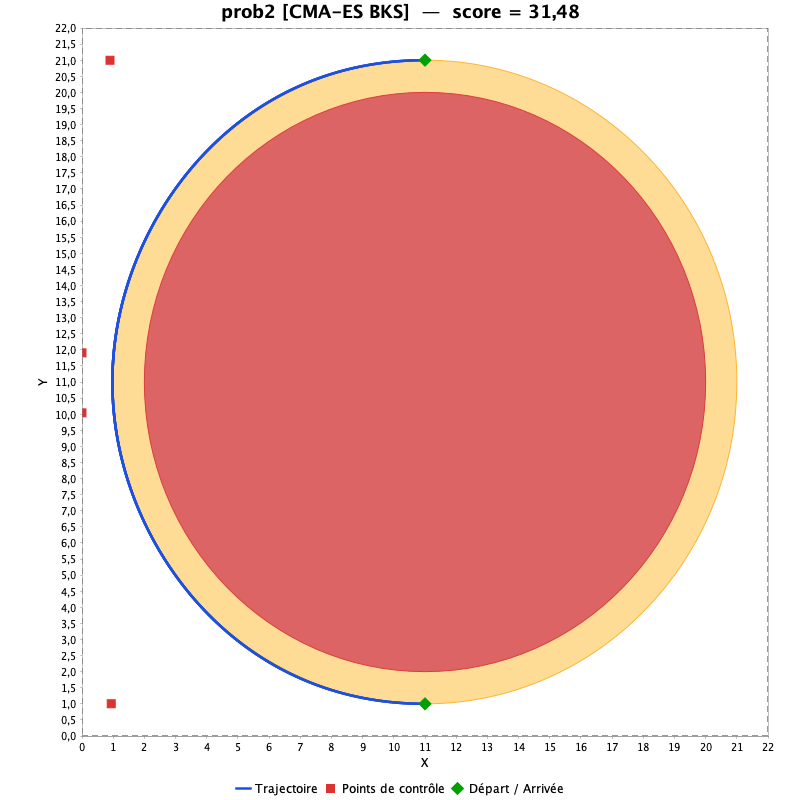
\includegraphics[width=\textwidth]{figures/bks/cmaes_prob2.png}
  \caption*{\small CMA-ES}
\end{subfigure}
\hfill
\begin{subfigure}{0.31\textwidth}
  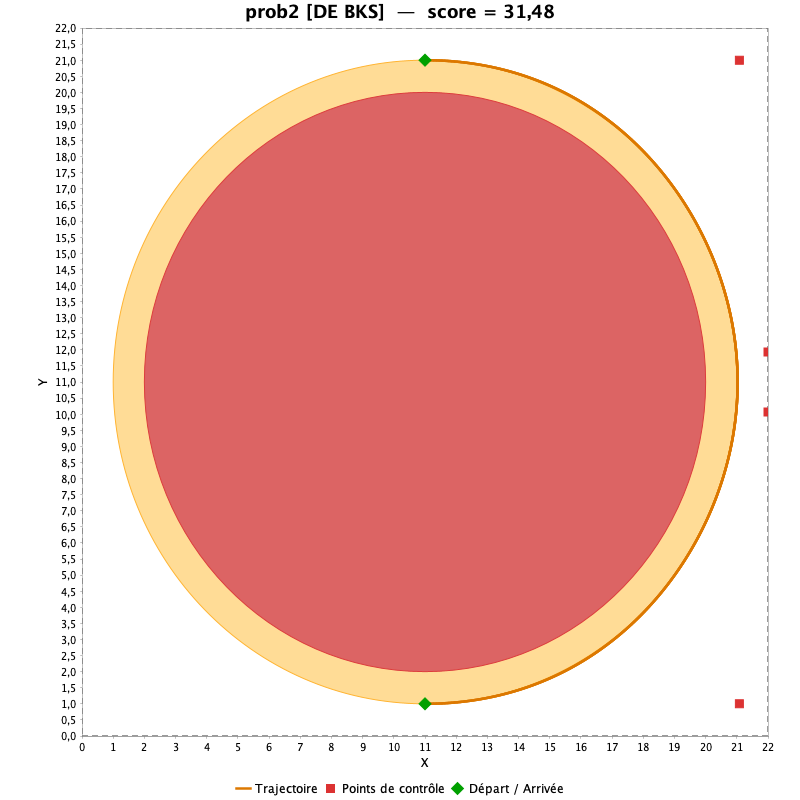
\includegraphics[width=\textwidth]{figures/bks/de_prob2.png}
  \caption*{\small DE}
\end{subfigure}
\hfill
\begin{subfigure}{0.31\textwidth}
  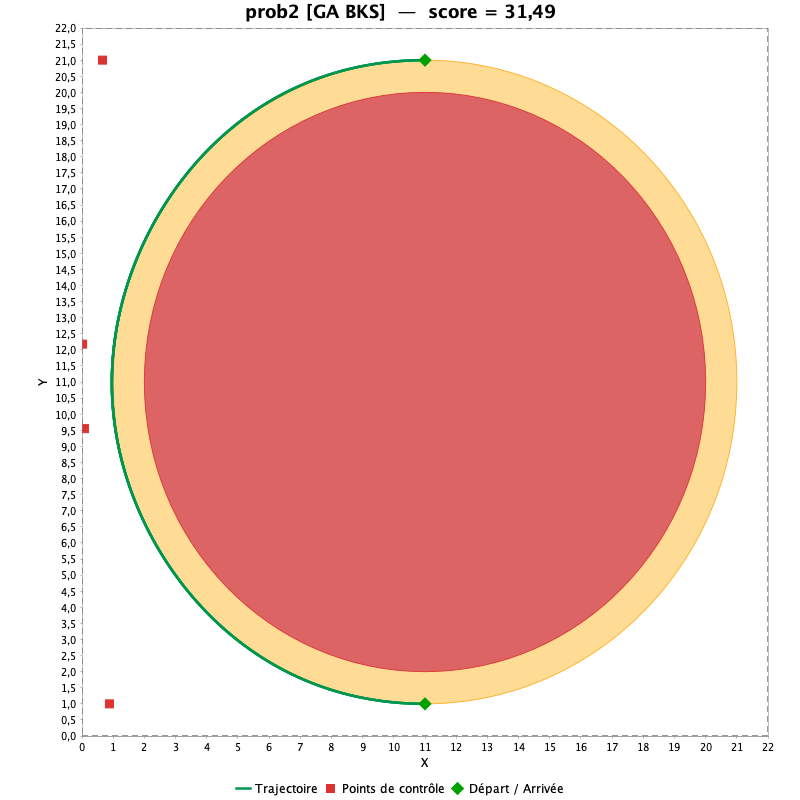
\includegraphics[width=\textwidth]{figures/bks/ga_prob2.png}
  \caption*{\small GA}
\end{subfigure}
\caption{\texttt{prob2} — Solutions BKS.}
\label{fig:bks_prob2}
\end{figure}

\begin{figure}[H]
\centering
\begin{subfigure}{0.31\textwidth}
  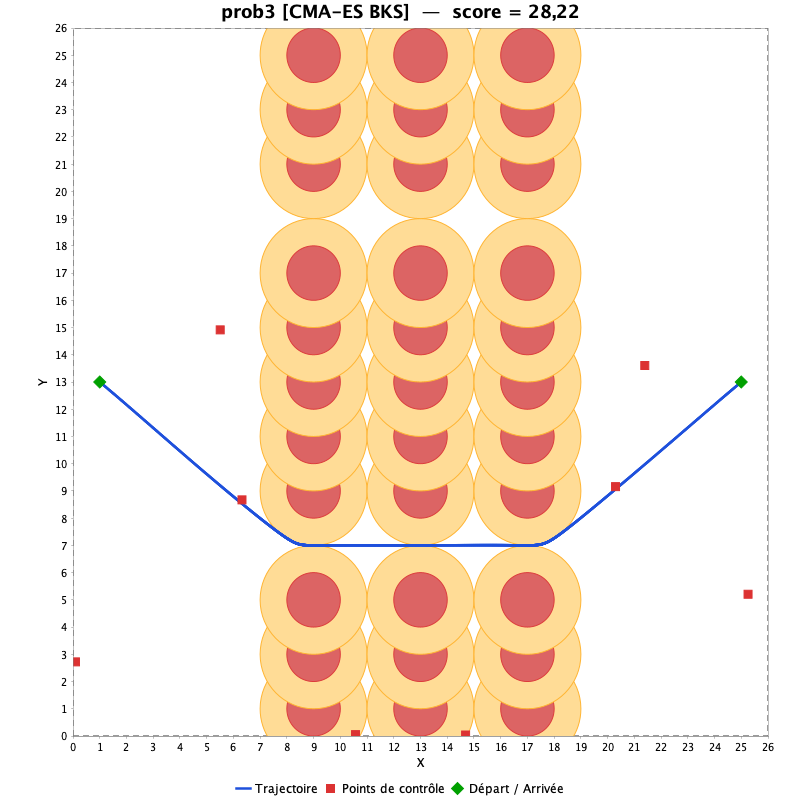
\includegraphics[width=\textwidth]{figures/bks/cmaes_prob3.png}
  \caption*{\small CMA-ES}
\end{subfigure}
\hfill
\begin{subfigure}{0.31\textwidth}
  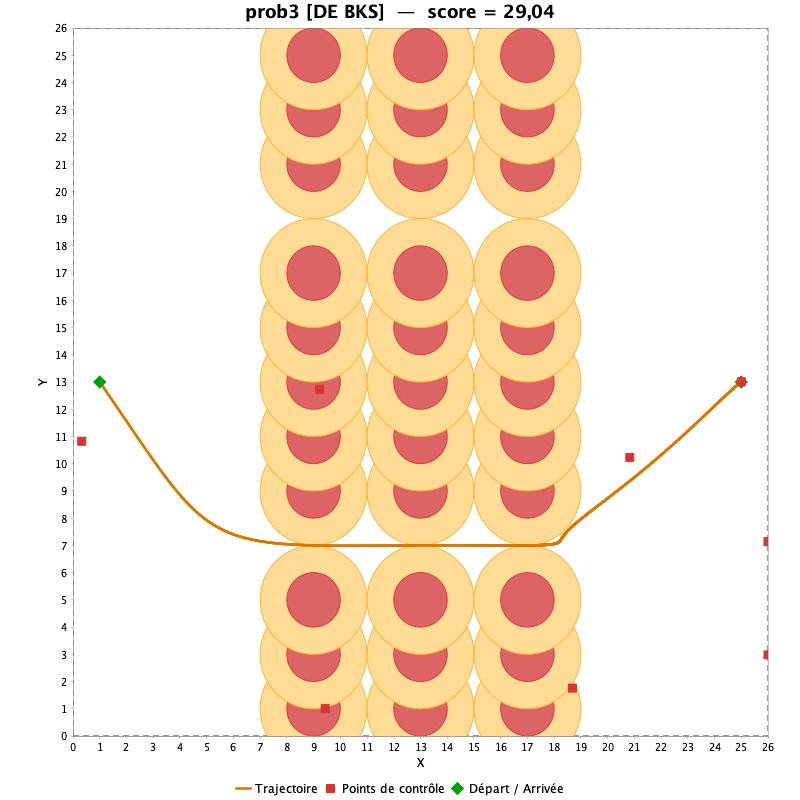
\includegraphics[width=\textwidth]{figures/bks/de_prob3.png}
  \caption*{\small DE}
\end{subfigure}
\hfill
\begin{subfigure}{0.31\textwidth}
  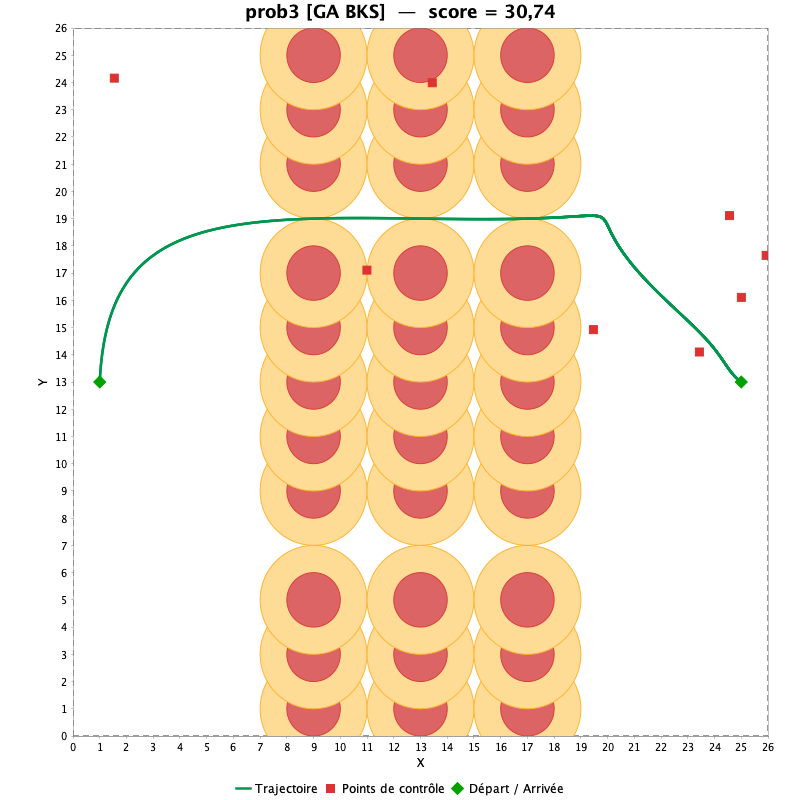
\includegraphics[width=\textwidth]{figures/bks/ga_prob3.png}
  \caption*{\small GA}
\end{subfigure}
\caption{\texttt{prob3} — Solutions BKS.}
\label{fig:bks_prob3}
\end{figure}

\begin{figure}[H]
\centering
\begin{subfigure}{0.31\textwidth}
  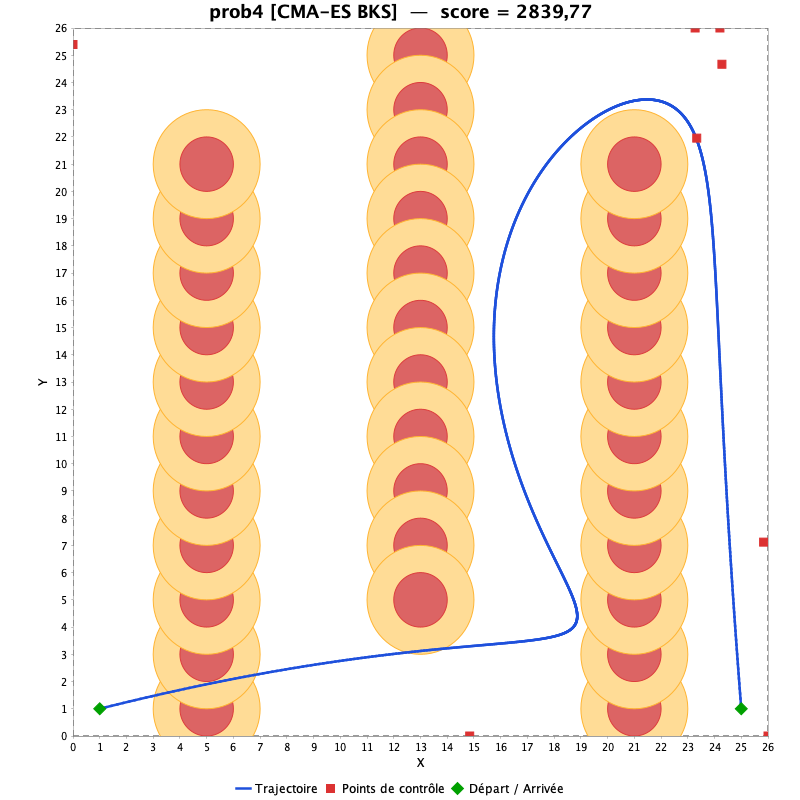
\includegraphics[width=\textwidth]{figures/bks/cmaes_prob4.png}
  \caption*{\small CMA-ES}
\end{subfigure}
\hfill
\begin{subfigure}{0.31\textwidth}
  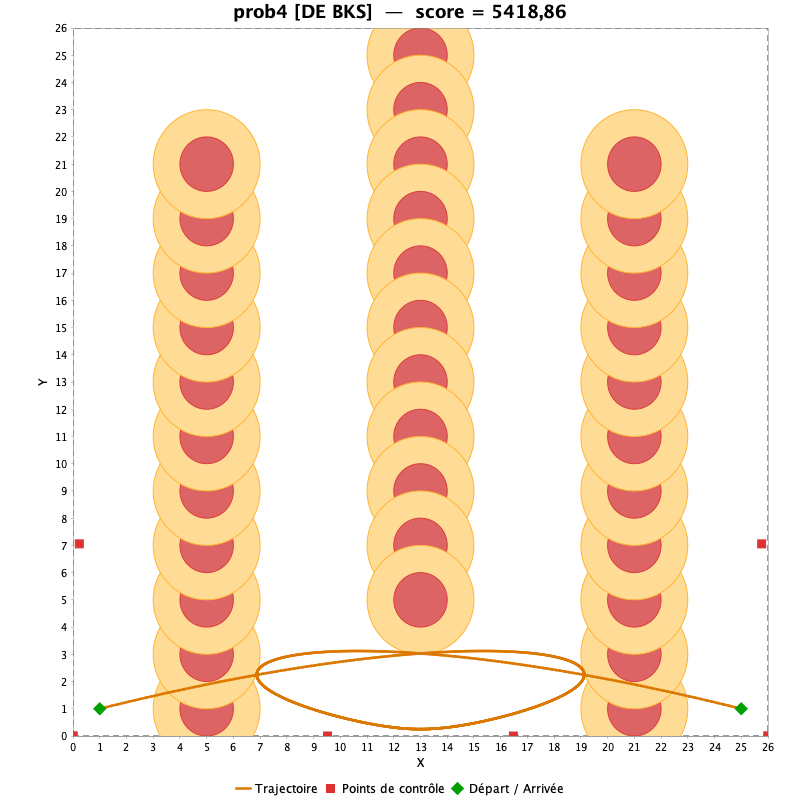
\includegraphics[width=\textwidth]{figures/bks/de_prob4.png}
  \caption*{\small DE}
\end{subfigure}
\hfill
\begin{subfigure}{0.31\textwidth}
  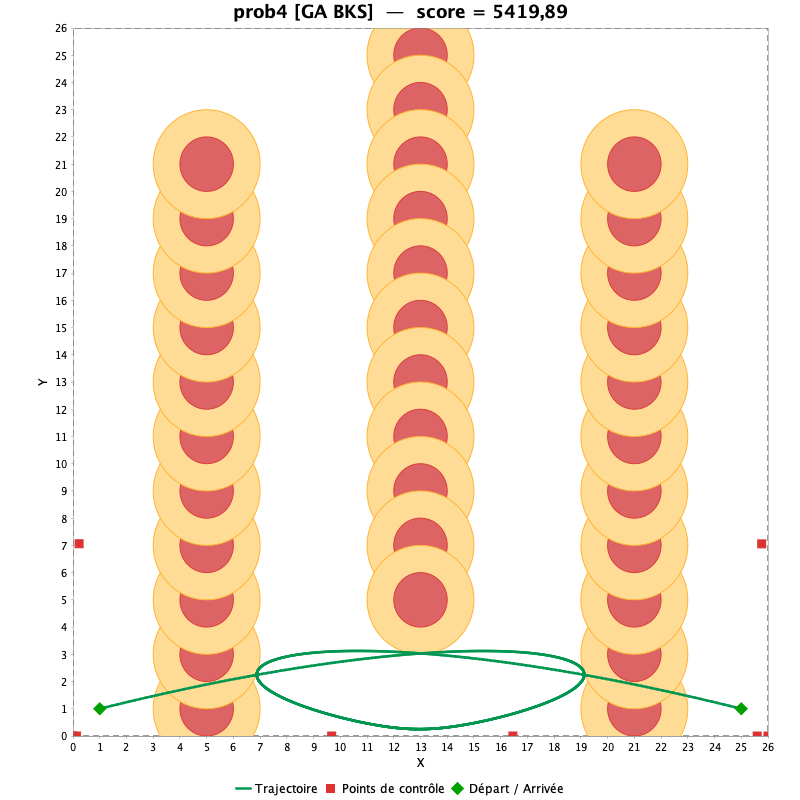
\includegraphics[width=\textwidth]{figures/bks/ga_prob4.png}
  \caption*{\small GA}
\end{subfigure}
\caption{\texttt{prob4} — Solutions BKS.}
\label{fig:bks_prob4}
\end{figure}
